\chapter{Úvod}
%\addcontentsline{toc}{chapter}{Úvod}

Strategické hry jsou žánrem, ve kterém hráči využívají svých mentálních schopností, především taktického a strategického myšlení, pro porážku jednoho či více nepřátel. Ve většině případů se strategické hry zabývají tématem války. \citep{book:gamefund}

Žánr strategických her obsahuje mnoho poddruhů s velice rozdílnými nároky jak na hráče, tak na vývojové prostředí a na vývojáře samotného. Prvním kritériem pro rozdělení strategických her je, zda se hra odehrává jako posloupnost diskrétních tahů, nebo zda se hra odehrává v přímé závislosti na ubíhajícím reálném čase. Druhým kritériem je relativní četnost a důležitost strategických rozhodnutí vůči taktickým rozhodnutím. Podle těchto dvou kritérií rozlišujeme tyto poddruhy:
\begin{itemize}
	\item Real-time strategy (RTS)
	\item Real-time tactics (RTT)
	\item Turn-based strategy(TBS)
	\item Turn-based tactics (TBT)
\end{itemize}

Real-time strategy (RTS) hry, v překladu strategické hry probíhající v reálném čase, jsou poddruhem strategických her ve kterém se změny stavu odehrávají v přímé závislosti na změně času v reálném světě. Reakce v reálném čase jsou náročnější jak pro hráče, který je často nucen použít suboptimální strategii, tak pro hru samotnou, která musí provádět výpočet dalšího stavu v omezeném čase. Stejně tak umělá inteligence, jakožto součást hry, musí reagovat na aktivity zbylých hráčů s omezeným časem, což limituje množství dat a složitost výpočtu, které může umělá inteligence použít. Z tohoto důvodu je vývoj RTS her složitým procesem, spojujícím mnoho oborů. Naším cílem je vytvořit platformu zjednodušující tvorbu těchto her.

 \footnote{Název "real-time strategy", poprvé použitý při propagaci hry Dune II, je připisován prezidentu a spoluzakladateli Westwood Studios, \emph{Brettu Sperrymu}. Toto studio následně využilo zkušenosti získané při tvorbě Dune II pro vývoj jedné z nejznámějších sérií RTS her, Command \& Conquer.}

Zbylé poddruhy strategických her neplánujeme v naší platformě explicitně podporovat, ale nijak nevylučujeme, že bude možné do jisté míry využít naší platformu i pro tvorbu těchto poddruhů strategických her. Zároveň je pro tvorbu RTS her výhodné znát příbuzné žánry, z kterých je možno se inspirovat a přebírat některé z jejich mechanik. Z tohoto důvodu ve zkratce popíšeme i zbylé poddruhy.

Prvním příbuzným žánrem jsou Real-time tactics (RTT) hry, někdy také nazývány fixed-unit real-time hry \citep{site:stratg02}, neboli hry s pevným počtem jednotek probíhající v reálném čase. Hlavním rozdílem, odlišující RTT od RTS, je omezení  strategických rozhodnutí a větším důrazem na taktická rozhodnutí a micromanagement jednotlivých jednotek. RTT hry nedovolují hráči tvorbu nových jednotek, stavbu budov či produkci surovin, hráč je tedy nucen s jednotkami, které má na začátku souboje, vyhrát celý souboj.  Jedním z příkladů čistě RTT her je série Blitzkrieg. Hráč začíná každou misi s jednotkami, které si vybral před misí. Tyto jednotky jsou jediné, které bude moci v průběhu mise využít, což nutí hráče použít svých taktických schopností a maximalizovat účinnost těchto jednotek. 

Turn-based strategy jsou strategické hry, ve kterých změny stavu probíhají v diskrétních tazích. Doba mezi tahy často není nijak omezena, což hráči umožňuje vymyslet optimální strategii. Oproti RTS tyto hry často omezují taktickou část a umožňují hráči soustředit se výhradně na strategickou část hry, tedy plánování budov, produkci surovin, vývoj technologií a celkovou strategii pro jeho ekonomiku a armádu. Příkladem tohoto žánru je série her Civilisation\citep{site:civ5}. \todo{popsat Civilisation} Naše platforma nebude explicitně podporovat tahy, myslíme si však, že bude možné toto rozdělení do tahů vytvořit použitím platformou poskytovaných \todo{něčeho}.


Turn-based tactics umožňují hráči přímé ovládání několika málo jednotek, které v každém tahu mohou provést jeden či více úkonů. Těmito úkony mohou být střelba na nepřátelskou jednotku, vyléčení přátelské jednotky, pohyb po mapě či například zničení terénu. Ukázkovým příkladem je série her X-COM. Ve hře X-COM 2 hráč vlastní až malé desítky jednotek, z kterých vybírá malou skupinu a vysílá ji na jednotlivé mise. Při misi má každá jednotka v každém tahu možnost vykonat dvě akce. Akce může být přesun o omezenou vzdálenost, použití schopnosti či útok na nepřítele. Pro normální jednotky útok ukončuje tah dané jednotky a hráč může provést tah následující. 



\section{RTS hry blíže}
Jak bylo řečeno výše, naše platforma bude navržena pro podporu vývoje RTS her. RTS hry jsou ovšem stále příliš velká množina s příliš rozmanitými mechanikami her na to, aby jedna platforma dokázala podporovat všechny možné RTS hry. Proto zde dále omezíme námi podporovanou podmnožinu RTS her.

Již od svého vzniku na konci osmdesátých let a začátku devadesátých let minulého století \todo{jiný slovo než obsahovaly} obsahovaly RTS hry několik konceptů, které lze nalézt v drtivé většině her tohoto žánru i dnes. 

Těmito koncepty jsou:
\begin{itemize}
	\item Výroba a ovládání jednotek s cílem ovládnutí části mapy a zničení nepřátelských jednotek a budov
	\item Stavba budov pro umožnění stavby nových druhů budov, jednotek či získání surovin
	\item Získávání surovin pro stavbu jednotek a budov
	\item Výzkum nových technologií
\end{itemize}

Základním stavebním kamenem RTS her je pečlivé vyvážení kombinace strategie/macromanagementu a taktiky/micromanagementu. Tyto pojmy bývají často špatně chápány a někdy zaměňovány, pokusíme se je proto konkrétně definovat. Strategií míníme \todo{citace} rozhodnutí týkající se globálního průběhu hry. Taktika \todo{citace} naopak zahrnuje konkrétní pozice konkrétních jednotek, jejich pohyb po mapě a spolupráci v jedné bitvě. 

Mezi strategická rozhodnutí v RTS hrách patří kupříkladu které budovy hráč postaví, v jakém pořadí dané budovy postaví, které suroviny bude produkovat, které suroviny vynechá, které jednotky bude rekrutovat a které vynechá. \todo{mozna graf nasledujiciho, jak se ovlivnujou} Tato 3 rozhodnutí jsou úzce propojena, protože výběr surovin určuje budovy, které bude hráč schopen postavit a typy jednotek, které bude moci zrekrutovat. Stejně tak výběr budov určuje suroviny, které hráč může produkovat a typy jednotek, které může zrekrutovat. 

Taktika/micromanagement je v RTS hrách reprezentován ovládáním jednotek, jejich přesné pozice, pohybu, směru útoku, používání schopností atd. Micromanagement lze ale vidět i v ekonomické stránce hry, kdy hráč 

Nejlepším příkladem pro rozlišení pojmu strategie a taktiky je série her Total War, které kombinuje mód tahové strategie s módem real-time tactics (RTT). V jedné části hry hráč přebírá kontrolu nad celým svým národem, rozhoduje, které budovy budou ve kterých městech postaveny, které jednotky budou rekrutovány a kde budou které armády umístěny. V druhé části, při souboji nepřátelských armád, hráč přebírá kontrolu nad konkrétní armádou a ovládá jednotlivé bataliony, jejich umístění, pohyb a útoky v reálném čase.

Naše platforma nemá za cíl nijak omezovat možnosti vytvářených her v rámci jejich zaměření na taktiku či strategii. Toto rozhodnutí chceme nechat čistě na uživateli naší platformy.


Hlavní inspirací pro tvorbu platformy, a tím i pro typ her, které bude platforma nejjednodušeji podporovat, byla hra Stronghold Crusader. Na této hře, vydané v roce 2002, ukážeme blíže základní principy RTS her a námi podporované implementace.

\subsection{Mapy}
Reprezentace herní mapy je jedním z hlavních rozhodnutí při tvorbě RTS her. Hlavní funkcí herní mapy je reprezentovat terén pro pohyb jednotek a stavbu budov. 
Tato funkce může zahrnovat neprostupné části mapy, několik různých druhů terénu prostupné různým druhům jednotek či části mapy ovlivňující rychlost pohybu jednotek.
Budovy jsou často omezeny typem terénu, na kterém je hráč schopen danou budovu postavit. Vzhledem k uzavřenosti většiny RTS her je složité zjistit, jak je v každé z nich herní svět reprezentován, z pozorovatelného vnějšího chování lze ale odvodit několik základních druhů reprezentací. 

Nejstarší a nejjednodušší reprezentací je rozdělení mapy na stejně velké dlaždice. Tyto dlaždice mohou být různých tvarů, nejčastěji jsou však čtvercové či hexagonální. Příkladem takovéto reprezentace je právě hra Stronghold Crusader, podle které chceme naši platformu modelovat. Jak je vidět na \ref{fig:tiletype}, herní mapa je viditelně rozdělena na stejně velké čtvercové dlaždice. Každá dlaždice má určen typ, který určuje její vzhled. Dále je tento typ využíván jako omezení při stavbě budov, kde například kamenolom lze postavit pouze na dostatečném počtu dlaždic typu kámen. Jak můžete vidět na \ref{fig:tiletype} poskytuje hra při stavbě budovy zpětnou vazbu v podobě  Na každé dlaždici může být postavena až na výjimky nejvýše jedna budova a stát nejvýše jedna jednotka. Při pohybu jednotek není tato vlastnost dodržována, lze tedy jednotky přesouvat přes dlaždice na kterých již jiná jednotka stojí. 

Naše platforma bude podporovat rozšířenější verzi tohoto druhu mapy, ve které nebudeme vynucovat limity na počty jednotek a budov na jedné dlaždici. Tato omezení budou přenechána pro implementaci tvůrcem her využívajících naší platformu a bude vytvořeno rozhraní pro co nejjednodušší implementaci těchto limitů.
\subsection{Jednotky}
Jednotky jsou základním nástrojem hráče pro boj s nepřítelem. Pohybem po mapě, poškozováním ostatních jednotek a ničením budov jednotky umožňují hráči vést souboj s protivníkem, získat strategickou výhodu a následně vyhrát hru. 

Hlavním odlišujícím prvkem od budov je možnost pohybu. Pohyb jednotky je určen jejím typem, kde každý typ jednotky může procházet jinými typy terénu, pohybovat se nad terénem, na vodě či pod vodou. Naše platforma bude podporovat pohyb jednotek kdekoli nad terénem, navíc bude tvůrcům poskytnuta komponenta umožňující chůzi po terénu, neboť je to nejčastější způsob pohybu. 

Pohyb jednotek je nejčastěji řízen hráčem, ať už na úrovni příkazů jednotlivým jednotkám, tak na úrovni slučování jednotek do skupin a ovládání těchto skupin. Naše platforma bude umožňovat jak ovládání jednotlivých jednotek, tak celých skupin. Dále umožníme vývojáři přidat složitější ovládání, například slučování do permanentních formací a následné ovládání těchto formací. 

V některých hrách existují také jednotky, které se mohou své schopnosti pohybu vzdát a stát se budovu, buď dočasně, nebo trvale. Příkladem takovéto jednotky je \todo{priklad a popsat ho}. Naše platforma by měla takovéto jednotky/budovy také podporovat. 

Ve velké části RTS her jsou jednotky schopny do určité míry autonomního rozhodování bez zásahu hráče, od střelby na cíl, který se ocitne v jejich dostřelu, po vyhledání krytu, pokud jsou pod palbou. 

Jako příklad jednoduché umělé inteligence jednotek můžeme vzít hry Starcraft a Warcraft od společnosti Blizzard. Zde se jednotky chovají velice předvídatelně, splňují přesně hráčovi rozkazy a nedělají nic navíc, což umožnilo hře Starcraft II vytořit jednu z prvních masivních e-sport scén na světě. \citep{gamasutra01}

Dobrým příkladem jednotek s vysokou autonomií je série Company of Heroes, kde jednotky automaticky vyhledávají krytí, rozutečou se, pokud jsou pod palbou dělostřelectva, a v případě příliš velkých ztrát utečou z boje. Tato autonomie má ale svou cenu, a to v nepředvídatelnosti chování jednotek. Při jednoduché umělé inteligenci jednotek je hráč schopen předvídat jejich chování a využít ho pro svůj prospěch. Naopak při složité umělé inteligenci, jako právě v případě Company of Heroes, je hráč často nucen provést více pokusů při vydávání rozkazu, protože není schopen jednoduše odhadnout chování jednotky. Tato skutečnost činí hry často realističtější, protože simuluje chování reálných vojáků, kteří rozkaz interpretují a implementují podle svého, není ale vhodná pro souboje více hráčů, a už vůbec né více hráčů na profesionální úrovni.

Platforma bude umožňovat vykonat libovolný kód v rámci každého výpočtu stavu každé jednotky, bude tedy pouze na vývojáři, zda se budou jednotky chovat jednoduše a předvídatelně, nebo zda budou vykonávat složité, avšak nepředvídatelné úkony bez hráčova vědomí. Pro ulehčení vývoje bude platforma poskytovat předpřipravené komponenty, umožňující základní úkony jako střelbu na cíl, pohyb po mapě a útok na blízko.

Jednou z vlastností definujících RTS hry je možnost produkce nových jednotek. Existuje několik systémů produkce jednotek, úzce svázaných se systémem surovin v dané hře. \todo{see Suroviny} Od kontinuální produkce, kde hráč zvolí produkované jednotky a suroviny jsou spotřebovávány v průběhu produkce, po diskrétní produkci, kde hráč musí vlastnit všechny suroviny potřebné pro výrobu dané jednotky při začátku produkce a všechny suroviny jsou odečteny v jeden okamžik. Kontinuální systém umožňuje hráči naplánovat produkci armády v předstihu, i když v daném okamžiku nevlastní dostatečné suroviny. Naopak při diskrétní produkci je hráč nucen čekat do chvíle, kdy má všechny suroviny, a až poté může začít s produkcí. Naše platforma se pokusí podporovat oba systémy. Bude záležet pouze na tvůrci hry, jak se k surovinám a produkci jednotek zachová a který z těchto systémů bude implementovat.

Počet jednotek je často limitován, jak pro účely vyvážení hry, tak pro omezení zátěže hardwaru. Z hlediska vyvážení síly jednotek umožňuje limit na počet jednotek předejít tzv. ``Zergu'', kdy hráč vytvoří obrovské množství levných jednotek, které následně převálcují jakýkoli odpor. Z hlediska hardwarové náročnosti je účel limitu vcelku zřejmý, protože každá jednotka zabírá určité množství paměti a výpočetního výkonu. Stronghold Crusader omezuje počet jednotek na 1000 pro každého hráče. Toto omezení se jeví především jako limit na hardwarovou náročnost hry. Naše platforma žádné explicitní limity nestanovuje, avšak v uživatelské dokumentaci pro vývojáře budeme silně doporučovat stanovení limitů na počet budov, jednotek a projektilů. Za tímto účelem umožníme vývojáři při vytvoření každé jednotky, budovy či projektilu rozhodnout se, zda je vytvoření možné a případně toto vytváření zrušit. 

Hráč často začíná s malým počtem jednotek, jejichž účelem je zamezit tzv. Rush strategii, ve které je cílem vytvořit co nejrychleji co možná nejvíce levných jednotek a zničit nepřítele ještě před tím, než je schopen začít produkovat své jednotky. Ve hře Stronghold Crusader například hráč začíná každou hru s několika lučišníky a kopiníky, jejichž počet je určen v nastavení před začátkem hry. Toto bude v naší platformě umožněno přidáváním jednotek v rámci editace mapy, případně pro počty jednotek určované před začátkem hry bude poskytnuta obrazovka, kde bude tvůrce hry schopen umístit grafické elementy pro nastavení, a následně při začátku hry vytvořit požadované množství jednotek. Tyto jednotky bude poté hráč vlastnit již na počátku hry.

V drtivé většině RTS her mají jednotky tzv. ``hit pointy'', zkráceně \textit{HP}, které určují počet zásahů, které může jednotka obdržet než bude zabita. S každým zásahem jsou poté tyto \textit{HP} odečítány a v okamžiku, kdy je jednotka poškozena na 0 \textit{HP} je zabita. Naše platforma bude tento systém samozřejmě podporovat, ale nebude ho nijak explicitně vyžadovat, bude tedy umožněno hráči použít jakýkoli jím implementovaný systém. 

Jednotky mohou obdržet poškození z mnoha zdrojů, nejčastěji však útokem z blízka (tzv. \textit{meele}) či z dálky (tzv. \textit{ranged}) jiné jednotky. Útok na blízko je omezen dosahem jednotky, rychlostí útoků a velikostí uděleného poškození. Naše platforma bude podporovat komponentu poskytující útoky na blízko právě s těmito parametry. Útok na dálku lze rozdělit do dvou typů, tzv. \textit{hit-scan} a \textit{projektily}. První typ je reprezentován například laserovými zbraněmi, které v okamžiku výstřelu urazí jakoukoli vzdálenost, dokud nenarazí na terén či nějakou entitu (budovu či jednotku). Druhý typ v okamžiku výstřelu vytvoří projektil, který se v průběhu času pohybuje herním světem, dokud také nenarazí na terén či nějakou entitu. Naše platforma bude podle předlohy Strongholdu Crusader podporovat především projektilové útoky. Za tímto účelem bude vytvořena komponenta umožňující střelbu projektilů, dále projektily samotné, simulace jejich letu a především možnost výpočtu pro střelbu na pohyblivý cíl. 

\subsection{Budovy}
Stavba budov představuje jednu z hlavních prezentací hráčovi strategie. Podle postavených budov lze často vcelku přesně odhadnout, jakou strategii hráč zvolil, čímž je umožněno nepřátelům reagovat a adaptovat svou strategii odpovídajícím způsobem. 

Hlavním rozdílem odlišujícím budovy od jednotek je 


V některých hrách existují budovy umožňující jednotkám pohybovat se po nich. Jak můžeme vidět na obrázku \ref{fig:unitsonbuildings} ze hry Stronghold Crusader, jednotky mohou být umístěny na hradbách, věžích, bránách či na tvrzi. Jak bylo řečeno v části o jednotkách, naše platforma bude umožňovat neomezený pohyb jednotkami, tedy i ve vzduchu, na budovách či skrz budovy. Protože se pohyb po budovách vyskytuje ve velkém množství RTS her, poskytne platforma možnost rozšíření terénu o plochu budov a komponentu umožňující chůzi po těchto plochách.

Umístění na budovách poskytuje jednotkám ochranu před nepřátelskými jednotkami útočícími na blízko, které se musí nejdříve dostat do blízkosti cíle, než zaútočí. 

V některých hrách, kde bohužel Stronghold Crusader není jednou z nich, poskytuje vyvýšení nad terén jednotkám větší dostřel. Tento efekt nemusí být omezen pouze na vyvýšení pomocí budov, ale lze ho dosáhnout už při rozdílných výškách terénu, na kterém je umístěn střelec a jeho cíl, obecněji na rozdílu výšky pozice střelce a cíle, pokud se střelec nemusí pohybovat přímo po terénu. Naše platforma bude podporovat realistické chování projektilů splňující tuto vlastnost. 

Budovy jsou často uspořádány do postupně se zlepšujících úrovní, které jsou zpřístupňovány výzkumem nových technologií. \todo{see Výzkum technologií} Každá z úrovní obsahuje řadu rozdílných budov, umožňujících zvolit různé strategie. Platforma bude umožňovat tvůrci  

Při této volbě lze ale narazit na problém, kdy je hráč nucen zvolit svou strategii před tím, než nalezne protivníky a tedy před tím, než může vidět jejich strategii. Tento problém je velmi výrazný při tzv.  ``rock-paper-scisors'' strategiích, kde strategie 1 poráží strategii 2, strategie 2 poráží strategii 3 a strategie 3 poráží strategii 1. V tuto chvíli hra degeneruje v loterii, zda hráč náhodně vybere správnou strategii porážející tu vybranou nepřítelem. Pro prevenci tohoto problému mají často  počáteční úrovně strategií pouze malé rozdíly v síle, což umožní hráčům reagovat a změnit svoji strategii před tím, než je rozdíl mezi jejich silami neúnosně velký. \citep{oxeye03} Dalším možným řešením, použitým ve Stronghold Crusader, je neskrývat před hráčem nepřítelovy akce. Toto řešení lze použít v různé míře, od odhalení nepřátelských budov po úplné odkrytí celé mapy, tedy pozice všech jednotek i budov, ať už přátelských, nepřátelských či neutrálních. Naše platforma použije toto poslední řešení.

Funkce budov:
\begin{itemize}
	\item Produkce jednotek
	\item Vylepšování jednotek
	\item Produkce surovin
	\item Uskladnění surovin
	\item Obrana
	\item Stavba budov
	\item Zkoumání technologií
\end{itemize}

\todo{rozepsat funkce}
Naše platforma se pokusí co nejvíce zjednodušit implementaci těchto funkcí, ale samotnou koncovou implementaci přenecháme až na tvůrce hry. Některé z těchto funkcí budou přenechány čistě pro implementaci tvůrcem hry, neboť ovlivňují pouze chování jednotek, do kterého naše platforma nebude nijak zasahovat.

Příkladem funkcí přenechaných pro implementaci tvůrci hry budou vylepšování jednotek, uskladnění surovin a zkoumání technologií. Pro jejich implementaci bude tvůrci poskytnut volný přístup ke grafickému rozhraní, do kterého může zobrazovat libovolná okna a jiné elementy.

Jak již bylo řečeno v \todo{makeref} sekci o jednotkách, naše platforma bude nechávat volbu mezi kontinuální a diskrétní produkcí jednotek na tvůrci hry. Budeme se tedy snažit do co největší míry podporovat oba tyto způsoby. 

Obrana bude podporována v podobě komponent, které umožní budovám jak útok na blízko, jako v případě pastí ve hře Stronghold Crusader, tak na dálku, jako například obranné věže ve hře Warcraft 3. 


\done
\todo{restrikce na umístění}

Budovy mají často restrikce, které je hráč nucen splnit před stavbou budovy. Tyto restrikce mohou sahat od reliéfu a typu terénu, přes existenci jiných budov ve stejném místě, po vlastnictví určitého množství surovin či typu jednotek. Naše platforma umožní tvůrci před stavbou budovy zjistit stav všech těchto typů restrikcí a případně vetovat stavbu budovy. 

Existující hry využívají několik možností, jak hráči poskytnout zpětnou vazbu o splnění restrikcí při stavbě budovy. Jednoduší možností, použitou ve hře Stronghold Crusader, je zobrazení půdorysu v různých barvách podle splnění restrikcí. Další, složitější možností je zobrazení průhledného či jinak upraveného modelu budovy na místech, kde ji nelze postavit.  Naše platforma bude podporovat jednoduší způsob, tedy zobrazení půdorysu budovy v různých barvách podle požadavků tvůrce hry.

\done
\todo{zničitelnost}
\done
\todo{různé druhy poškození}

Budovy, podobně jako jednotky, mají ve většině her určitý počet tzv. ``hit pointů'', které určují počet zásahů, které může budova obdržet před tím, než bude zničena. Navíc oproti jednotkám mohou budovy často obdržet poškození pouze od omezené podmnožiny jednotek, nejčastěji pouze obléhacích strojů. Stejně jako u jednotek přenecháme systém poškození na tvůrci hry. Naše platforma pouze umožní budově reagovat na zásah projektilem či zbraní, ať už snížením svých \textit{HP}, nebo ignorováním daného útoku v případě že přišel od jednotky či projektilu, který danou budovu nemůže poškodit.

\subsection{Suroviny}
Resource management je přítomný ve všech hrách tohoto žánru již od jeho vzniku. Od koření v Dune II, přes zlato a dřevo ve Warcraft 3, po všechny typy surovin ve hře Stronghold, získávání surovin je jednou z hlavních motivací konfliktu v RTS hrách. 

Systémy surovin lze rozdělit podle způsobu získávání a počtu typů surovin.

Podle způsobu získávání můžeme systém surovin rozdělit na
\begin{enumerate}
	\item Aktivní získávání surovin
	\item Pasivní získávání surovin
\end{enumerate}

Při aktivním získávání surovin existuje ovladatelná herní entita, která svým pohybem mezi pozicemi na mapě přináší suroviny. Tento pohyb může být ovládán hráčem, ale nejčastěji dokáže pracovat jednotka samostatně. Příkladem může být Warcraft 3, kde speciální jednotky získávají dřevo a zlato přenášením z lesů/dolů do hráčovy hlavní budovy.

Při pasivním získávání přibývají suroviny bez akcí entit, pouze díky vlastnictví určité části mapy nebo druhu budovy. Zdroj bývá nekonečný nebo skoro nekonečný, poskytující suroviny do obsazení nebo zničení zdroje.

Každý z těchto stylů podporuje jinou strategii kontroly mapy.

Naše platforma bude podporovat jak pasivní, tak aktivní získávání surovin. Bude pouze na tvůrci, v jakém okamžiku budou suroviny přičteny, ať už v závislosti na čase nebo na pohybu určitých jednotek. 

\subsection{Vývoj technologií}
Volba vyzkoumaných technologií důležitou součástí strategické části RTS her. 

Technologie jsou často uspořádány ve stromové struktuře, kde vyzkoumání technologie v rodičovském uzlu odemyká technologie ve svých synech. Každé větvení představuje možné rozhodnutí hráče, kterou z větví bude dále zkoumat. V některých hrách bývají dokonce větve výlučné, tedy vyzkoumání jedné větve zamkne přístup k vyzkoumání jiné větve.

Vyzkoumání technologie může mít mnoho různých efektů. Nejčastějším efektem bývá odemknutí nového typu jednotek nebo budov. Další možností je změna vlastností již vlastněných jednotek nebo budov. V neposlední řadě pak může vyzkoumání technologie odemknout nové schopnosti nebo kouzla, které hráč může následně použít při taktických soubojích. 

\begin{figure}[h]
	\label{fig:civ5techtree}
	\caption{Výřez stromu technologií ze hry Civilisation V}
	\centering
	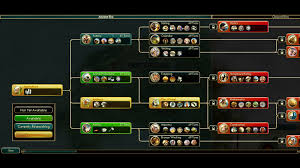
\includegraphics{civ5_tech_tree}
\end{figure}


\begin{figure}[h]
	\label{fig:warcrafttechtree}
	\caption{Budovy a závislosti mezi nimi tvořící obdobu stromu technologií ve hře Warcraft 3}
	\centering
	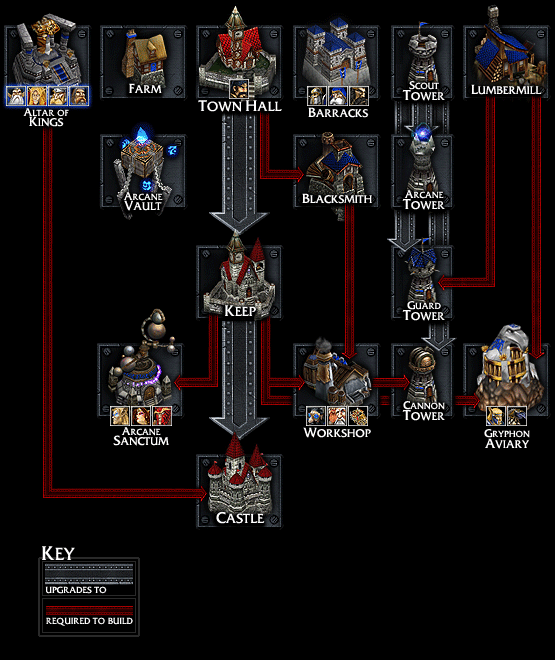
\includegraphics{warcraft_tech_tree}
\end{figure}

Explicitní strom technologií, přítomný např. ve hrách série Civilisation, se v RTS hrách vyskytuje spíše výjimečně. Nejčastěji je odemykání nových typů jednotek a budov umožněno stavbou určitého typu budovy nebo dosažení určitého stupně vylepšení již existující budovy. Jako příklad můžeme vzít Warcraft 3, kde závislosti budov na stupních vylepšení a existenci jiných budov tvoří strom technologií. 

Jak bylo řečeno v sekci o budovách, 


\section{Požadavky}
V předešlé sekci jsme popsali druh her, které bude naše platforma podporovat, jejich vlastnosti a restrikce. V této sekci popíšeme požadavky na chování platformy všech druhů našich uživatelů.

\subsection{Tvůrci her}
Prvním druhem uživatele budou tvůrci RTS her, používající naši platformu pro zjednodušení své práce a vyřešení problémů opakujících se ve většině RTS her. Tvůrce her samozřejmě nemusí být pouze jeden člověk, vzhledem ke složitosti RTS her existuje při jejich tvorbě mnoho rolí s různými požadavky na různé schopnosti, které může plnit více lidí. Příkladem rolí může být 3D umělec tvořící modely a animace, producent hudby, tvůrce umělé inteligence, programátor herní logiky a nakonec člověk, který toto vše integruje dohromady.

Naším hlavním cílem je umožnit tvůrcům umělé inteligence a programátorům herní logiky použít všechny jazyky .NET Frameworku, a především C\#, pro jejich práci. Z jejich pohledu bude naše platforma sloužit jako knihovna poskytující tyto funkce:

\begin{enumerate}
	\item Dotazovat se na aktuální stav hry
	\item Vytvářet nové jednotky, budovy a projektily
	\item Registrovat si metody, které budou zavolány při určitých událostech v průběhu hry
	\item Upravovat terén
	\item Vykreslovat terén, jednotky, budovy, projektily a grafické rozhraní
	\item Ukládat a načítat stav hry
	\item Implementace pro základní problémy jako pohyb po terénu, let projektilů, výpočet při střelbě projektilů, \todo{more}
\end{enumerate}

Protože implementace vykreslování a grafického rozhraní by byla nad rámec jedné bakalářské práce, využije naše platforma pro tyto účely herní engine UrhoSharp. Pro programátory následně platforma poskytne přístup k relevantním částem UrhoSharp enginu.

Pro integraci všech částí bude naše platforma umožňovat vytvořit \emph{balíček}, obsahující vše vytvořené programátory a umělci.  Tento balíček poté platforma umožní přidat a načíst v libovolné instalaci platformy.

Platforma bude také sloužit jako editor úrovní, které budou využívat logiku a assety dodané pomocí balíčků. Vytvořené úrovně bude následně možné uložit zpět do balíčku a distribuovat spolu s balíčkem do dalších instancí naší platformy.

Pro editaci mapy poskytne platforma několik základních nástrojů a umožní tvůrcům modifikovat základní nástroje či přidávat své vlastní. Základní nástroje by měli umožnit přinejmenším editaci terénu mapy (změnu typu terénu na všechny tvůrci definované typy a editaci výšky v rozlišení na jednotlivé rohy dlaždic) a přidávání všech druhů jednotek a budov.

Formát ukládání úrovní bude definován otevřeně pomocí prostředků nezávislých na programovacím jazyce, čímž chceme umožnit tvorbu separátních editorů map produkujících úrovně v námi používaném formátu.

\todo{Kamera}

\subsection{Hráči her}
Pro hráče se bude platforma chovat jako instalovatelná aplikace, která hráči umožní za běhu přidávat balíčky a tyto balíčky dále použít.

Při běhu platforma umožní plný přístup k nastavení UrhoSharp enginu, tedy k nastavení rozlišení atd.\todo{more params}.


\todo{more}

\section{Ukázková hra}

Pro ukázku bude vytvořena jednoduchá hra, demonstrující možnosti našeho frameworku. 

Ukázková hra bude obsahovat několik jednotek, demonstrujících tyto vlastnosti:
\begin{enumerate}
	\item Jednoduchou a složitou umělou inteligenci
	\item Plně automatické jednotky, neovladatelné hráčem
	\item Jednotky útočící na dálku
	\item Jednotky útočící na blízko
	\item Aktivní získávání surovin
	\item Pohyb po terénu
	\item Pohyb nad terénem (létání)
	\item Rozdílnou rychlost pohybu různých jednotek
	\item Rozdílnou přístupnost částí mapy pro různé jednotky
	\item Pohyb po budovách
\end{enumerate}

Demonstrovanými vlastnostmi budov budou:
\begin{enumerate}
	\item Restrikce na místo stavby
	\item Neprostupnost budov pro některé jednotky
	\item Produkce surovin budovami
	\item Přidání plochy nebo části plochy budovy jako přístupný terén pro určité typy jednotek
\end{enumerate}

Jako obecné vlastnosti bude ukázková hra demonstrovat:
\begin{enumerate}
	\item RTS mód kamery
	\item Volný pohyb kamery
	\item Sledování jednotky kamerou
	\item Tvůrcem definované prvky v uživatelském rozhraní
	\item Minimapu
\end{enumerate}

\section{Cíle práce}
Cílem této práce je vytvořit framework pro vývoj 3D RTS her pro jednoho hráče, umožňující vývojářům vytvářet hry jako separátně 
distribuované balíčky, které bude poté koncový uživatel schopen přidat do našeho frameworku nainstalovaném na uživatelově počítači a použít pro hraní dodaných úrovní či tvorbu svých vlastních.

Při tvorbě balíčků bude umožněno tvůrci použít jazyky frameworku .NET  pro vytvoření Umělé inteligence jednotek, budov a nepřátelských hráčů, další logiky hry a pro přidání nástrojů do editoru map.

Požadované vlastnosti frameworku:
\begin{enumerate}
	\item Vlastnosti pro tvůrce balíčků:
		\begin{enumerate}
			\item Framework musí umožňovat přidávání balíčků za běhu, obsahujících nové typy jednotek, budov,  dlaždic, projektilů a hráčů spolu s jejich modely, texturami a AI.
			\item Framework musí umožňovat použití přidaných balíčků pro tvorbu map a uložení vytvořených map do balíčku použitého pro jejich vytvoření
			\item Editor map musí být rozšiřitelný pomocí pluginů z balíčku.
			\item Herní user interface musí umožňovat rozšiřitelnost pro tlačítka, okna a další grafické prvky přidávané tvůrcem.
		\end{enumerate}

	\item Vlastnosti pro koncového hráče:
		\begin{enumerate}
			\item User interface pro stolní počítače, umožňující vybírání balíčků, map a oponentů, dále načítání a ukládání her, a nastavování zobrazení hry.
			\item Herní user interface musí obsahovat minimapu, poskytující hráči přehled o větší části mapy než kterou vidí vlastní kamerou.
			\item Ovládání kamery umožňující klasický top-down pohled, volné poletování kamery po mapě a následování jednotky
			\item Ukládání a načítání hry
		\end{enumerate}
\end{enumerate}
